% Chapter 1

\chapter{Findings} % Main chapter title

\label{findingschapter} % For referencing the chapter elsewhere, use \ref{Chapter1} 

\lhead{Chapter 1. \emph{Research Findings}} % This is for the header on each page - perhaps a shortened title

%----------------------------------------------------------------------------------------

\section{Pilot Evaluation II Findings}
\subsection{Baseline}
We had a total of sixteen participants who completed the baseline questionnaire. There were two sets of participants. The first set consisted of seven beneficiaries while the second set consisted of nine intermediaries. At baseline level, findings are both in form of descriptive and inferential statistics. These findings focus on comparison between participants' characteristics from the two aforementioned sets.  \newline
At baseline, I examined three out of five variables, and these were age of participants, number of services/applications utilized by each participant, and intrinsic motivation to use cellphone. Other variables only existed in one group, therefore lacked comparative basis. The findings based on these variables is reported at mid-line and end-line points sections. \newline
Table \ref{table:ageDist} shows the mean age with its respective standard deviation for each set of participants. Beneficiaries had a mean age of 48 years old (SD: 7.9 years) while intermediaries had a mean age of 14 years (SD: 4.3 years).
\newline
\begin{table}[h!]
  \begin{center}
    \caption{Age distribution of two sets of participants at baseline.}
    \label{table:ageDist}
	\begin{tabular}{|r|r|r|r|}
		\hline
		Types of Users& Sample Size (n)& Mean age& Standard Deviation\\
		\hline
		Beneficiary Users& 7& 48.29& 7.910\\
		\hline
		Intermediary Users& 9& 14.00& 4.272\\
		\hline
	\end{tabular}
  \end{center}
\end{table}
\newline
The distribution of age in both sets was normal. I conducted a student t test to compare means of age from the two sets(groups). The mean age of intermediaries' set was significantly lower (M=14 ; SD=4.27) years compared to beneficiaries' set(M= 48.29; SD=7.910) years with (t(14)=11.148; p$<$0.01; 95\% CI= -40.88 to -27.69 years ). The mean difference in age was 34.28 years with a standard error of 3.08 years.
\newline
As part of the baseline questionnaire, I provided a list of names of cellphone based services/applications(apps) for participants to choose from. The words applications and services are used interchangeably throughout this chapter. The list contained ten services as demonstrated on Table \ref{table:servTab}. This list is not exhaustive but it attempted to capture most services that are considered to be prevalent.  
\begin{table}[h!]
  \begin{center}
    \caption{List of services/apps in the baseline questionnaire.}
    \label{table:servTab}
{ \renewcommand{\arraystretch}{1.2}
\begin{tabular}{|l|x{2cm}|x{10cm}|}
\hline
{}& \textbf{Service name}& \textbf{Description and purpose}\tn \hline
         1& SMS& SMS stands for short messaging service. It is one of the basic feature in every phone It is used for communication purposes \tn \hline
         2& Downloading& It is an Internet based service of where people download files such as music and video.\tn \hline
         3& WhatsAPP& Internet based messaging application.It is used for communication purposes \tn \hline
		 4& BBM& Internet based messaging application typically found in blackberry phones. It is used for communication purposes \tn \hline
		 5& WhatsAPP& Internet based messaging application. It is used for communication purposes \tn \hline
		 6& Facebook& Internet based social network platform which enables individuals to have social interactions \tn \hline
		 7& Twitter& Internet based social network platform which enables individuals to have social interactions \tn \hline
		 8& Email& It is an Internet based platform that allows individuals to have formal or informal communication. \tn \hline
		9& Pedometer& It refers to a specialized device or an application installed on mobile devices such as
		cellphones. Its purpose is to sense bodily movements. It is has to be attached to a person's body typically on the waist or at the front pocket of a trouser. An advanced pedometer can transfer detected movements via Internet or Bluetooth. It is recommended for tracking exercise or activity routines. \tn \hline
		10& Diary for Diet& It refers to an electronic journal that can be used to track meals eaten and probably provide summaries on which users can reflect on. It can installed either on stationary medium such as a personal computer or mobile devices such as cellphones, tablets, PDAs etc. \tn \hline
\end{tabular} }
 \end{center}
\end{table}
\newline Each participant selected services/app they have either interacted with before or they are knowledgeable with. Figure \ref{figure:OverallSerBase} indicates that SMS and Camera were the most prevalent with comparison to the remaining applications or services considering the number of participants that were using them. All sixteen participants indicated that they had interacted with both SMS and Camera before
\begin{figure}[htbp]
  \centering
    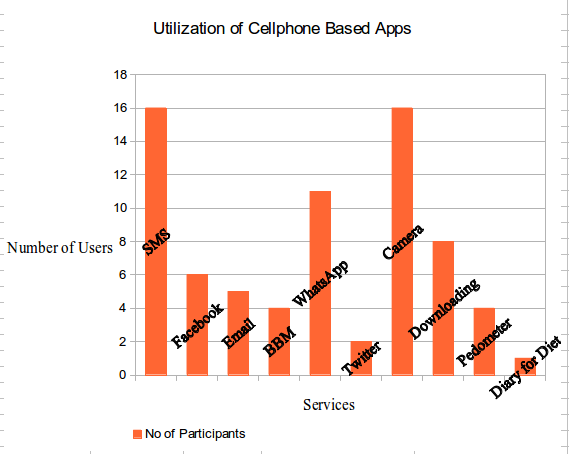
\includegraphics[width=0.8\textwidth]{Figures/overallcellphoneusebaseline.png}
    \rule{35em}{0.5pt}
  \caption{Average utilization of services and apps by the two groups of participants.}
  \label{figure:OverallServBase}
\end{figure}
\begin{figure}[htbp]
  \centering
    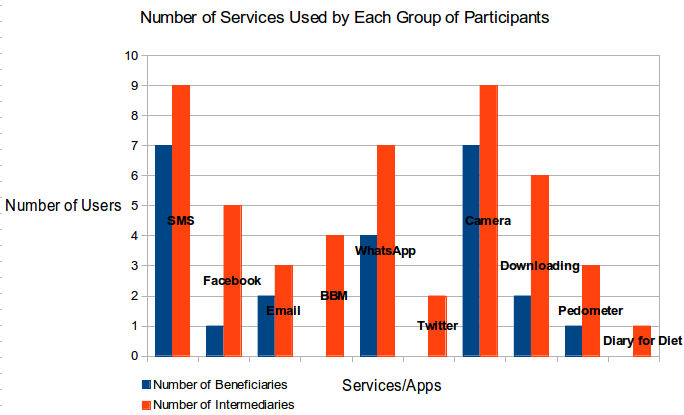
\includegraphics[width=0.8\textwidth]{Figures/baselinepilotallservices.png}
    \rule{35em}{0.5pt}
  \caption{Average utilization of services and apps by the two groups of participants.}
  \label{figure:AllServBase}
\end{figure}
I conducted a further analysis that compares the number of services the two groups of participants have interacted with before. Figure \ref{figure:AllServBase} shows the number of participants from each set that have interacted with each of the aforementioned services on Table \ref{table:servTab} above.
Figure \ref{figure:AllServBase} was not a good indicator of any differences between the two sets because the two samples differed in their sizes. I made a decision to only compare the averages of number of services used by each group of participants. Figure \ref{figure:AvgServBase}  shows that there is a difference on the averages of number of services that intermediaries have interacted with compared to the number of services beneficiaries have interacted with.
\begin{figure}[htbp]
  \centering
    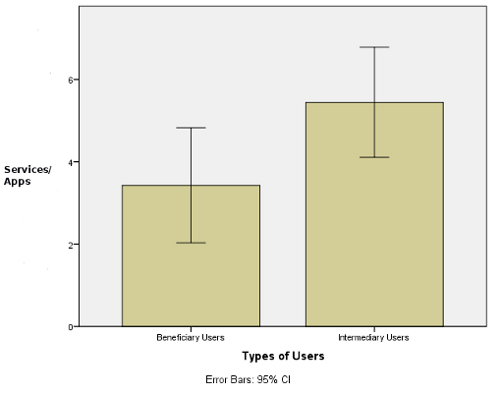
\includegraphics[width=0.8\textwidth]{Figures/ServicesBaseline.png}
    \rule{35em}{0.5pt}
  \caption{Average utilization of services and apps by the two groups of participants.}
  \label{figure:AvgServBase}
\end{figure}
A further inferential analysis by using a student t test indicated that intermediary participants had significantly interacted with more applications (M=5.44; SD=1.74) applications more of the aforementioned services compared to beneficiary users (M=3.43; SD=1.51) applications (t(14)=2.430; p=0.029; 95\% CI=3.765 to 3.795 applications). Due to a small sample size, I was unable to conduct a statistical test to compare the average usage of each service/application between intermediary and beneficiary participants.\newline
The above findings on average number of apps used by each group of participants suggest that our intermediary participants are more likely to interact with more services or applications compared to our beneficiary participants. These findings were in consensus with the observed difference in intrinsic motivation to use cellphone between the two groups. Figure 2 below shows a cluster bar chart for each scale I used for calculating the overall "{\textbf{\emph{intrinsic motivation to use cellphone}}". Figure \ref {figure:IMIScales} presents a descriptive visualization of differences in individual scales of intrinsic motivation to use cellphone in between intermediaries and beneficiaries.    
\begin{figure}[htbp]
  \centering
    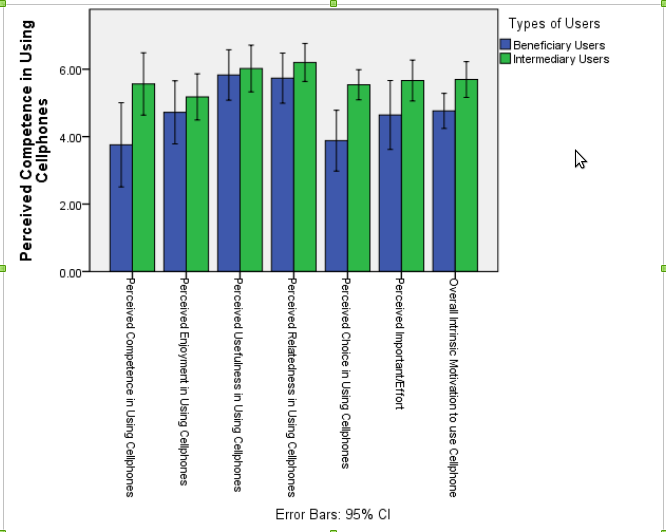
\includegraphics[width=0.8\textwidth]{Figures/IMIScales.png}
    \rule{35em}{0.5pt}
  \caption{Average utilization of services and apps by the two groups of participants.}
  \label{figure:IMIScales}
\end{figure}  
I conducted a student t-test to examine whether intermediaries and beneficiaries had significant differences on both scores from individual scales and overall intrinsic motivation. On scores of individual scales,  the differences were not significant in perceived enjoyment; perceived usefulness; and perceived relatedness. There were significant differences on the following scales; perceived competence; perceived choice; and perceived effort. Intermediaries scored significantly higher on perceived competence to use cellphones (M=5.5611 ;SD=1.20254) compared to beneficiaries (M=3.7571 ;SD=1.35106) with conditions;(t(14)=2.822 ; p=0.014 ; 95\% CI=0.43307 to 3.17486). Intermediaries' perception on self autonomy(perceived choice) to use cellphone (M=5.5378 ;SD=0.57933 ) was significantly higher compared to beneficiaries' perceived choice to use cellphone (M=3.8814;SD=0.97472) with conditions (t(14)=4.247; p=0.001; 95\% CI=0.81984  to 2.49286 ). Also intermediaries (M=5.6633; SD=0.78889) scored significantly higher on perceived effort/important compared to beneficiaries (M=4.6429 ;SD=1.10583) with conditions (t(14)=2.159; p=0.049; 95\% CI=0.00670 to 2.03426).\newline
On comparison between an overall intrinsic motivation scores to use cellphone between the two groups, intermediaries(M=5.6944 ;SD=0.69013 ) scored significantly higher than beneficiaries(M=4.7629 ;SD=0.56287) with conditions (t(14)=2.894; p=0.012; 95\% CI=0.24123 to 1.62194).These findings indicate that intermediary participants were more intrinsically motivated to engage with cellphones compared to beneficiary participants.
\begin{flushright}
\end{flushright}
